%-------------------------------------------------
%
% Generator.tex
%
%------------------------------------------------
\section[Generatori di dati]{generatori di dati}
\label{pt1:generator}
Al fine di ottenere una discreta quantità di dati su cui effettuare dei test si è progettato e conseguentemente implemento, in linguaggio $C++$,
un programma in grado di generare diverse tipologie di istanze.

Il programma è composto da alcuni oggetti di servizio che hanno lo scopo di rappresentare gli oggetti della realtà da studiare (\texttt{Plate} e \texttt{Hole}).

Tra le componenti più importanti troviamo quelle che consentono di generare i punti secondo una specifica strategia, ovvero le seguenti:

\begin{itemize}
\item\texttt{PlateGenerator}: classe base che fornisce la possibilità di generare delle piastre con le coordinate dei fori;
\item\texttt{RandomPlateGenerator}: fornisce l'algoritmo per la generazione di punti casuali su di una superficie di dimensioni date;
\item\texttt{ClusterPlateGenerator}: fornisce l'algoritmo per la generazione di punti suddivisi in un numero di \english{cluster} fornito dall'utente;
\item\texttt{CirclePlateGenerator}: fornisce l'algoritmo per la generazione di punti su di un percorso circolare chiuso.
\end{itemize}

L'ultima componente è quella che consente di serializzare una piastra e salvarne i dati essenziali su \english{file} di testo, è composta dalle seguenti classi:

\begin{itemize}
\item\texttt{ProblemGenerator}: classe base che fornisce le funzionalità di salvataggio dei dati su \english{file} e fornisce la possibilità di generare i dati del problema.
\item\texttt{EuclideanProblemGenerator}: fornisce l'algoritmo per il calcolo delle distanze euclidee tra i singoli fori che compongono la piastra.
\end{itemize}

Viene ora fornita la struttura dei \english{files} che compongono tale programma.

\dirtree{%
.1 generator.
.2 src.
.3 header.
.4 generator.
.5 CirclePlateGenerator.h.
.5 ClusterPlateGenerator.h.
.5 EuclideanProblemGenerator.h.
.5 PlateGenerator.h.
.5 RandomPlateGenerator.h.
.4 object.
.5 Hole.h.
.5 Plate.h.
.3 source.
.4 generator.
.5 CirclePlateGenerator.cpp.
.5 ClusterPlateGenerator.cpp.
.5 EuclideanProblemGenerator.cpp.
.5 ProblemGenerator.cpp.
.5 RandomPlateGenerator.cpp.
.4 object.
.5 Hole.cpp.
.5 Plate.cpp.
.2 main.cpp.
.2 makefile.
}

In Figura \ref{pt1:generator:imgs} sono riportati alcuni esempi di dati generati attraverso le varie tipologie di generatore implementate:

\begin{figure}
\centering
\begin{subfigure}[b]{0.45\textwidth}
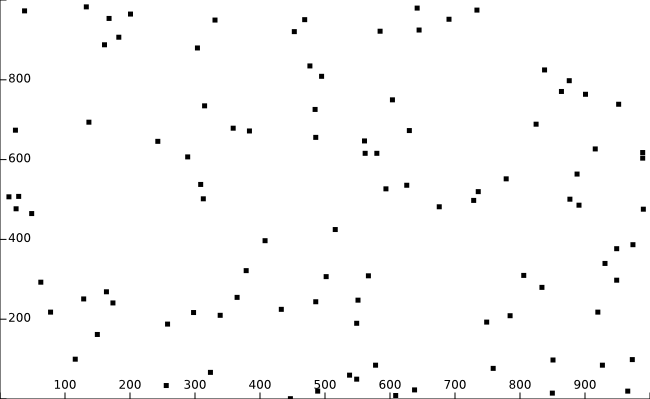
\includegraphics[width=\textwidth]{Images/Part_1/Instances/Random.png}
\caption{Random}
\label{pt1:generator:random_img}
\end{subfigure}
\quad{}
\begin{subfigure}[b]{0.45\textwidth}
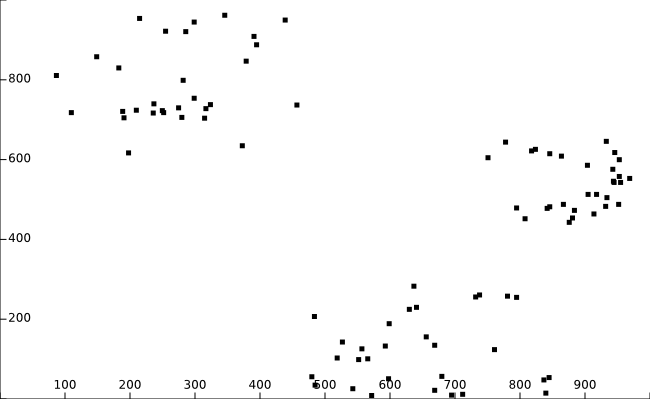
\includegraphics[width=\textwidth]{Images/Part_1/Instances/Cluster.png}
\caption{Cluster}
\label{pt1:generator:cluster_img}
\end{subfigure}

\begin{subfigure}[b]{0.5\textwidth}
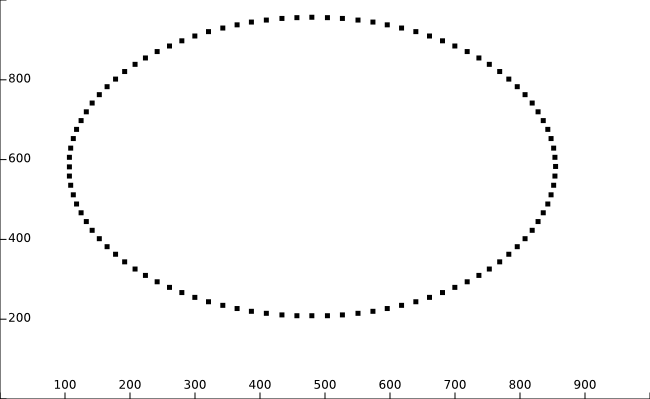
\includegraphics[width=\textwidth]{Images/Part_1/Instances/Circle.png}
\caption{Circuito}
\label{pt1:generator:Circle_img}
\end{subfigure}
\caption{Esempi di istanze generate}
\label{pt1:generator:imgs}
\end{figure}

Il programma produce due \english{files} per ogni istanza generata. Un \english{file}, con estensione \texttt{.crd}, contenente le coordinate dei punti generati ed un \english{file}, con estensione \texttt{.dat}, contenente i costi calcolati.

Per ottimizzare lo spazio di salvataggio si è deciso che, dati due nodi $i$ e $j$ nel \english{file} contenente i dati (\texttt{.dat}) viene salvato solamente il costo dell'arco $i,j$ in quanto l'arco inverso $j,i$ è deducibile dalla simmetria del grafo. Il \english{file} contiene nella prima riga il numero di fori generati e a seguire tutti i costi, uno per ogni riga.